

%% 2016/11/17
%% by Filippo Baldini



\documentclass[conference]{IEEEtran}
\usepackage{blindtext, graphicx}

\usepackage{caption}
\usepackage{subcaption}

\makeatletter
\def\subsubsection{\@startsection{subsubsection}% name
	{3}% level
	{\z@}% indent (formerly \parindent)
	{0.7ex plus 0.1ex minus 0.1ex}% before skip
	{0.7ex}%{0ex}% after skip
	{\normalfont\normalsize\itshape}}% style

\makeatother


% Add the compsoc option for Computer Society conferences.
%
% If IEEEtran.cls has not been installed into the LaTeX system files,
% manually specify the path to it like:
% \documentclass[conference]{../sty/IEEEtran}





% Some very useful LaTeX packages include:
% (uncomment the ones you want to load)


% *** MISC UTILITY PACKAGES ***
%
%\usepackage{ifpdf}
% Heiko Oberdiek's ifpdf.sty is very useful if you need conditional
% compilation based on whether the output is pdf or dvi.
% usage:
% \ifpdf
%   % pdf code
% \else
%   % dvi code
% \fi
% The latest version of ifpdf.sty can be obtained from:
% http://www.ctan.org/tex-archive/macros/latex/contrib/oberdiek/
% Also, note that IEEEtran.cls V1.7 and later provides a builtin
% \ifCLASSINFOpdf conditional that works the same way.
% When switching from latex to pdflatex and vice-versa, the compiler may
% have to be run twice to clear warning/error messages.






% *** CITATION PACKAGES ***
%
%\usepackage{cite}
% cite.sty was written by Donald Arseneau
% V1.6 and later of IEEEtran pre-defines the format of the cite.sty package
% \cite{} output to follow that of IEEE. Loading the cite package will
% result in citation numbers being automatically sorted and properly
% "compressed/ranged". e.g., [1], [9], [2], [7], [5], [6] without using
% cite.sty will become [1], [2], [5]--[7], [9] using cite.sty. cite.sty's
% \cite will automatically add leading space, if needed. Use cite.sty's
% noadjust option (cite.sty V3.8 and later) if you want to turn this off.
% cite.sty is already installed on most LaTeX systems. Be sure and use
% version 4.0 (2003-05-27) and later if using hyperref.sty. cite.sty does
% not currently provide for hyperlinked citations.
% The latest version can be obtained at:
% http://www.ctan.org/tex-archive/macros/latex/contrib/cite/
% The documentation is contained in the cite.sty file itself.






% *** GRAPHICS RELATED PACKAGES ***
%
\ifCLASSINFOpdf
  % \usepackage[pdftex]{graphicx}
  % declare the path(s) where your graphic files are
  % \graphicspath{{../pdf/}{../jpeg/}}
  % and their extensions so you won't have to specify these with
  % every instance of \includegraphics
  % \DeclareGraphicsExtensions{.pdf,.jpeg,.png}
\else
  % or other class option (dvipsone, dvipdf, if not using dvips). graphicx
  % will default to the driver specified in the system graphics.cfg if no
  % driver is specified.
  % \usepackage[dvips]{graphicx}
  % declare the path(s) where your graphic files are
  % \graphicspath{{../eps/}}
  % and their extensions so you won't have to specify these with
  % every instance of \includegraphics
  % \DeclareGraphicsExtensions{.eps}
\fi
% graphicx was written by David Carlisle and Sebastian Rahtz. It is
% required if you want graphics, photos, etc. graphicx.sty is already
% installed on most LaTeX systems. The latest version and documentation can
% be obtained at: 
% http://www.ctan.org/tex-archive/macros/latex/required/graphics/
% Another good source of documentation is "Using Imported Graphics in
% LaTeX2e" by Keith Reckdahl which can be found as epslatex.ps or
% epslatex.pdf at: http://www.ctan.org/tex-archive/info/
%
% latex, and pdflatex in dvi mode, support graphics in encapsulated
% postscript (.eps) format. pdflatex in pdf mode supports graphics
% in .pdf, .jpeg, .png and .mps (metapost) formats. Users should ensure
% that all non-photo figures use a vector format (.eps, .pdf, .mps) and
% not a bitmapped formats (.jpeg, .png). IEEE frowns on bitmapped formats
% which can result in "jaggedy"/blurry rendering of lines and letters as
% well as large increases in file sizes.
%
% You can find documentation about the pdfTeX application at:
% http://www.tug.org/applications/pdftex





% *** MATH PACKAGES ***
%
%\usepackage[cmex10]{amsmath}
% A popular package from the American Mathematical Society that provides
% many useful and powerful commands for dealing with mathematics. If using
% it, be sure to load this package with the cmex10 option to ensure that
% only type 1 fonts will utilized at all point sizes. Without this option,
% it is possible that some math symbols, particularly those within
% footnotes, will be rendered in bitmap form which will result in a
% document that can not be IEEE Xplore compliant!
%
% Also, note that the amsmath package sets \interdisplaylinepenalty to 10000
% thus preventing page breaks from occurring within multiline equations. Use:
%\interdisplaylinepenalty=2500
% after loading amsmath to restore such page breaks as IEEEtran.cls normally
% does. amsmath.sty is already installed on most LaTeX systems. The latest
% version and documentation can be obtained at:
% http://www.ctan.org/tex-archive/macros/latex/required/amslatex/math/





% *** SPECIALIZED LIST PACKAGES ***
%
%\usepackage{algorithmic}
% algorithmic.sty was written by Peter Williams and Rogerio Brito.
% This package provides an algorithmic environment fo describing algorithms.
% You can use the algorithmic environment in-text or within a figure
% environment to provide for a floating algorithm. Do NOT use the algorithm
% floating environment provided by algorithm.sty (by the same authors) or
% algorithm2e.sty (by Christophe Fiorio) as IEEE does not use dedicated
% algorithm float types and packages that provide these will not provide
% correct IEEE style captions. The latest version and documentation of
% algorithmic.sty can be obtained at:
% http://www.ctan.org/tex-archive/macros/latex/contrib/algorithms/
% There is also a support site at:
% http://algorithms.berlios.de/index.html
% Also of interest may be the (relatively newer and more customizable)
% algorithmicx.sty package by Szasz Janos:
% http://www.ctan.org/tex-archive/macros/latex/contrib/algorithmicx/




% *** ALIGNMENT PACKAGES ***
%
%\usepackage{array}
% Frank Mittelbach's and David Carlisle's array.sty patches and improves
% the standard LaTeX2e array and tabular environments to provide better
% appearance and additional user controls. As the default LaTeX2e table
% generation code is lacking to the point of almost being broken with
% respect to the quality of the end results, all users are strongly
% advised to use an enhanced (at the very least that provided by array.sty)
% set of table tools. array.sty is already installed on most systems. The
% latest version and documentation can be obtained at:
% http://www.ctan.org/tex-archive/macros/latex/required/tools/


%\usepackage{mdwmath}
%\usepackage{mdwtab}
% Also highly recommended is Mark Wooding's extremely powerful MDW tools,
% especially mdwmath.sty and mdwtab.sty which are used to format equations
% and tables, respectively. The MDWtools set is already installed on most
% LaTeX systems. The lastest version and documentation is available at:
% http://www.ctan.org/tex-archive/macros/latex/contrib/mdwtools/


% IEEEtran contains the IEEEeqnarray family of commands that can be used to
% generate multiline equations as well as matrices, tables, etc., of high
% quality.


%\usepackage{eqparbox}
% Also of notable interest is Scott Pakin's eqparbox package for creating
% (automatically sized) equal width boxes - aka "natural width parboxes".
% Available at:
% http://www.ctan.org/tex-archive/macros/latex/contrib/eqparbox/





% *** SUBFIGURE PACKAGES ***
%\usepackage[tight,footnotesize]{subfigure}
% subfigure.sty was written by Steven Douglas Cochran. This package makes it
% easy to put subfigures in your figures. e.g., "Figure 1a and 1b". For IEEE
% work, it is a good idea to load it with the tight package option to reduce
% the amount of white space around the subfigures. subfigure.sty is already
% installed on most LaTeX systems. The latest version and documentation can
% be obtained at:
% http://www.ctan.org/tex-archive/obsolete/macros/latex/contrib/subfigure/
% subfigure.sty has been superceeded by subfig.sty.



%\usepackage[caption=false]{caption}
%\usepackage[font=footnotesize]{subfig}
% subfig.sty, also written by Steven Douglas Cochran, is the modern
% replacement for subfigure.sty. However, subfig.sty requires and
% automatically loads Axel Sommerfeldt's caption.sty which will override
% IEEEtran.cls handling of captions and this will result in nonIEEE style
% figure/table captions. To prevent this problem, be sure and preload
% caption.sty with its "caption=false" package option. This is will preserve
% IEEEtran.cls handing of captions. Version 1.3 (2005/06/28) and later 
% (recommended due to many improvements over 1.2) of subfig.sty supports
% the caption=false option directly:
%\usepackage[caption=false,font=footnotesize]{subfig}
%
% The latest version and documentation can be obtained at:
% http://www.ctan.org/tex-archive/macros/latex/contrib/subfig/
% The latest version and documentation of caption.sty can be obtained at:
% http://www.ctan.org/tex-archive/macros/latex/contrib/caption/




% *** FLOAT PACKAGES ***
%
%\usepackage{fixltx2e}
% fixltx2e, the successor to the earlier fix2col.sty, was written by
% Frank Mittelbach and David Carlisle. This package corrects a few problems
% in the LaTeX2e kernel, the most notable of which is that in current
% LaTeX2e releases, the ordering of single and double column floats is not
% guaranteed to be preserved. Thus, an unpatched LaTeX2e can allow a
% single column figure to be placed prior to an earlier double column
% figure. The latest version and documentation can be found at:
% http://www.ctan.org/tex-archive/macros/latex/base/



%\usepackage{stfloats}
% stfloats.sty was written by Sigitas Tolusis. This package gives LaTeX2e
% the ability to do double column floats at the bottom of the page as well
% as the top. (e.g., "\begin{figure*}[!b]" is not normally possible in
% LaTeX2e). It also provides a command:
%\fnbelowfloat
% to enable the placement of footnotes below bottom floats (the standard
% LaTeX2e kernel puts them above bottom floats). This is an invasive package
% which rewrites many portions of the LaTeX2e float routines. It may not work
% with other packages that modify the LaTeX2e float routines. The latest
% version and documentation can be obtained at:
% http://www.ctan.org/tex-archive/macros/latex/contrib/sttools/
% Documentation is contained in the stfloats.sty comments as well as in the
% presfull.pdf file. Do not use the stfloats baselinefloat ability as IEEE
% does not allow \baselineskip to stretch. Authors submitting work to the
% IEEE should note that IEEE rarely uses double column equations and
% that authors should try to avoid such use. Do not be tempted to use the
% cuted.sty or midfloat.sty packages (also by Sigitas Tolusis) as IEEE does
% not format its papers in such ways.





% *** PDF, URL AND HYPERLINK PACKAGES ***
%
%\usepackage{url}
% url.sty was written by Donald Arseneau. It provides better support for
% handling and breaking URLs. url.sty is already installed on most LaTeX
% systems. The latest version can be obtained at:
% http://www.ctan.org/tex-archive/macros/latex/contrib/misc/
% Read the url.sty source comments for usage information. Basically,
% \url{my_url_here}.



% correct bad hyphenation here
\hyphenation{op-tical net-works semi-conduc-tor}


\begin{document}
%
% paper title
% can use linebreaks \\ within to get better formatting as desired
\title{Smartini: An Interactive, Learning-Capable, Cocktail-Making Robot}


% author names and affiliations
\author{
	Chantal Tognetti, Emanuele Gentili, Fabian Duffhauss, Filippo Baldini, Tim K. Chan\\
	{\tt\small \{ct2416, eg2214, fad16, fb1713\}@ic.ac.uk, timchan@berkeley.edu}\\
	Electrical \& Electronic Engineering Department, Imperial College London\\
}

% conference papers do not typically use \thanks and this command
% is locked out in conference mode. If really needed, such as for
% the acknowledgment of grants, issue a \IEEEoverridecommandlockouts
% after \documentclass

% for over three affiliations, or if they all won't fit within the width
% of the page, use this alternative format:
% 
%\author{\IEEEauthorblockN{Michael Shell\IEEEauthorrefmark{1},
%Homer Simpson\IEEEauthorrefmark{2},
%James Kirk\IEEEauthorrefmark{3}, 
%Montgomery Scott\IEEEauthorrefmark{3} and
%Eldon Tyrell\IEEEauthorrefmark{4}}
%\IEEEauthorblockA{\IEEEauthorrefmark{1}School of Electrical and Computer Engineering\\
%Georgia Institute of Technology,
%Atlanta, Georgia 30332--0250\\ Email: see http://www.michaelshell.org/contact.html}
%\IEEEauthorblockA{\IEEEauthorrefmark{2}Twentieth Century Fox, Springfield, USA\\
%Email: homer@thesimpsons.com}
%\IEEEauthorblockA{\IEEEauthorrefmark{3}Starfleet Academy, San Francisco, California 96678-2391\\
%Telephone: (800) 555--1212, Fax: (888) 555--1212}
%\IEEEauthorblockA{\IEEEauthorrefmark{4}Tyrell Inc., 123 Replicant Street, Los Angeles, California 90210--4321}}




% use for special paper notices
%\IEEEspecialpapernotice{(Invited Paper)}




% make the title area
\maketitle


\begin{abstract}
The purpose of our research and the making of the Smartini Cocktail Robot was to create an interactive and learning-capable robot that address the challenge of human-robot interaction and modern cocktail making through state-of-the-art technology. We explored different modes of communication, including eye-contact, gestures and speech. We included an entertainment system in our Smartini, composed of jokes and news telling. Smartini can also learn customer trends on the taste of the drinks and adjust its recipes accordingly. From the data we collected, customers were highly satisfied with the cocktail making process,  which scored 4.23/5. However Smartini's movements, eye-contact and easiness of communication rated 3.54/5. While these might have been the intrinsic limitations of the iCub's slow speed of motion and of the computational power of our computers, to make a truly functional and enjoyable Smartini robot these areas need to be improved.
\end{abstract}





% For peer review papers, you can put extra information on the cover
% page as needed:
% \ifCLASSOPTIONpeerreview
% \begin{center} \bfseries EDICS Category: 3-BBND \end{center}
% \fi
%
% For peerreview papers, this IEEEtran command inserts a page break and
% creates the second title. It will be ignored for other modes.
\IEEEpeerreviewmaketitle



\section{Introduction}

	The market for service robotics is constantly growing and is estimated to increase substantially in the next 20 years \cite{stats}\cite{stats2}. As more and more robots will become part of our daily lives, human-centred interaction is vital for human satisfaction. Hence, it is not enough for a robot to achieve task-based goals solely, but it should also satisfy the social aspect that arise through interaction with people in real-world settings. Building a robot with this purpose presents several challenges. In fact, not only does the robot require the abilities to recognise and understand human signals like gaze, facial expression, and languages especially , but also it would have to generate a realistic response using similar modalities. To address these challenges, we developed a bartender robot — Smartini — by building a system on top of the humanoid robot iCub in connection with an Arduino. The iCub is responsible for human-robot interaction. It also controls another machine through the system which was built around an Arduino to actually prepare the drink, like a coffee machine but with cocktail instead. Smartini can recognise humans as customers, initiate conversion, take their orders, and serve them drinks. Furthermore, the robot’s behaviour is controlled by an artificial brain. There are two fundamental interactions. On one hand, setting the robot to a task-only environment, where it simply prepares and serves drinks to human. On the other hand, it is expected to exhibit social behaviour that is derived from typical human interactions in a socially intelligent setting.

\section{Hypothesis}

We incorporated learning algorithms into Smartini that made it able to modify its behaviour based on customer feedback. In particular, we proposed the following hypotheses: 

\begin{itemize}
	\item
	Through the feedback-gathering system, Smartini will successfully adjust the cocktail recipes to customer trends, and the appreciation rate of the beverages will increase with time;
    \item
    The entertainment will have a positive impact on the customer experience, with targeted expressions and jokes about robotics and cocktails resulting in higher appreciation than more general, informative communication;
    \item
    Eye contacts and hand gestures will be perceived by the users as crucial for an enjoyable and natural experience.
    
\end{itemize}


\section{Previous Work}

\subsection{Human-Robot Interaction}

From the beginning of robotics, researchers have been exploring the possibility of interaction between a human and a robot, as well as a robot and its environment. This field of study has further expanded when biologically-inspired robots made their first appearance \cite{socialBots}.

The goal of socially interactive robots is to operate in place of human peers or assistants. Therefore, it is safe to assume that humans prefer to interact with such machines in the same way that they would interact with other people \cite{socialBots}. An analysis of human behaviours during verbal interactions must therefore be taken into account when developing our Smartini. For example, Sidner et al. \cite{engagement} showed that tracking the human face and moving the robot's head accordingly during a conversation is highly beneficial to the perceived quality of the interaction by the human user. Furthermore, users direct their attention to the robot more often in interactions where hand gestures occur with speech. Both these features can be incorporated in our design to improve  user experience. 

Previous attempts to design an interactive robot have shown different approaches. Kollar, Thomas, et al. \cite{mmodal} and Gockley, Rachel, et al. \cite{valeria} have both implemented a receptionist robot. This type of robot presents many similarities to our Smartini in terms of the hospitality functionality. Both a receptionist and a bartender stay relatively stationary behind either a desk or a bar table while talking with the customers. 

While Kollar et al. implemented multi-modal communication, based on the correct interpretation of face expressions and hand gestures, Gockley et al. adopted a simpler speech-only input, which is what we aim to implement given the time frame. 

A very important lesson can be learnt from Gockley, who programmed the receptionist to give lengthy monologues and found that few users stayed to hear more than 1–2 sentences of the story, due to the lack of interaction. We shall focus on providing a more natural dialogue with people.

Various consumer electronics companies are currently active in the entertainment robotic sector. In particular, Sony recently they produced various versions of dog-like robots (AIBOs) and the newer humanoid robot (SDR). When developing the AIBOs \cite{petRobot}, they invested particular attention to its `lifelike' appearance as a design principle. Sony argues that more realistic and real-life-like behaviours have a higher chance to trigger a response from the user, hence resulting in better entertainment. We have no control over the hardware design, but choosing the iCub as our platform we already ensured a human appearance of our robot. Our goal is therefore to develop our robot beyond a simple cocktail-making machine to a device closely resembling a bartender, able to ask questions, make jokes, tell stories etc. as a real bartender would do.

\subsection{Computer Vision}

Research in computer vision provided a variety of object detection and recognition approaches. Most of them attempt to recognise an object based on prior knowledge, which is often represented by labelled samples, or pairs of a sensory input with an interpretation \cite{c1}.

In the image processing field, prior knowledge can also take the form of algorithm choices or image databases, where each object is associated with several images or visual properties encoded by descriptors. In this case, object recognition relies on the similarity with existing database entities. This approach is fast and reliable, but it is not easily applicable for autonomous learning, where robots should construct adaptable object representations. This can be achieved by using dedicated interfaces, as proposed in \cite{c2}, that allow users to provide learning examples to the robot. For example, in \cite{c3}, the robot learns objects that are simply shown by the caregiver, whereas in \cite{c4} the robot performs tasks which are expected to reveal useful information about the objects in the scene. In \cite{c5}, finally, the robot performs simple actions (grasping, pushing, etc.) to learn the properties of items (e.g. a ball and a cylinder can roll).

Fast and robust real-time object localisation is also provided by algorithms detecting artificial markers. For instance, the ARTag system, widely used in virtual reality applications, creates and recognizes such markers \cite{c6}. However, this requires object tagging.

An efficient identification of specific object categories is also possible using numerous narrow-purpose detectors. Examples are face detectors \cite{c7} that work with low-level Haar-like features, and human skin detectors \cite{c8} that process the colour of pixels. The latter is also used to enhance image segmentation, by subtracting the regions of human hands holding objects \cite{c9}.

In terms of object localisation (subsequent to recognition), several approaches have previously been developed for the iCub platform. Pattacini (2011) created the \textit{cartesianController} module, which provides basic 3D position estimation functionality and gaze control. This module works well on the simulated iCub, however it is not fully supported and functional on the hardware platform, and therefore it does not perform well. Currently the most accurate available localisation module for the iCub is the \textit{stereoVision} module, which provides accuracy in the range of a few centimetres.

\subsection{Speech Recognition}

In extensive research projects in the 1950s and 1960s the first recogniser system were developed which was able to recognise vowels, phonemes, isolated numbers or monosyllabic words. Since these systems were trained and optimised for a certain speaker, the recognition accuracy dropped dramatically for other speakers \cite{SRhistory}.

A very important milestone was the investigation and application of linear predictive coding (LPC) and hidden Markov acoustic models (HMMs) for speech recognition in the 1970s. These methods enabled the automatically analysis of large quantities of speech data with little computation time and result in a highly improved recognition performance \cite{speechLP}, \cite{SRTechn}.

The first large-vocabulary speaker-independent continuous speech recognition system was demonstrated in 1988. This system called {\it Sphinx} is based on HMMs and LPC and has been improved since then \cite{Sphinx1988}. A modern successor of this recogniser is {\it PocketSphinx} \cite{PocketSphinx} which was used for the Smartini earlier.

\section{Design} \label{design}

In the early stages of our project, we discussed what functions the Smartini would carry out and how to implement them. Our goal was to obtain a robot that could understand an order, prepare the chosen cocktail, entertain the user as a human bartender would do while preparing the drink, and gather feedback on the quality of the beverage as well as the interaction, gradually learning and improving its performance with time. 

Initial research showed that the iCub  was able to handle cups and pour liquids \cite{pouringLiquids}, but would do so slowly and with some difficulty. Therefore we decided to ease the task of preparing the cocktail by minimising the movements to a minimum. Shaking the cocktail was the most complicated part, as multiple mechanical parts would have to move at the same time. Therefore we anticipated some testing to be done with different shaking techniques, involving one or two hands. 

We also addressed the issue of keeping the cup closed while shaking the beverage. This is done easily by a human bartender, but it would be an involved and dangerous task for a mechanical robot. We designed a 3D-printable shaker which has an magnetic cap with a electronic-switch that can be controlled by iCub. Moreover, the iCub would wear water-proof gloves to prevent any damage from spillage. 

However, when we presented this design to the supervisors in charge of the iCub, they advised us against it. They argued that the iCub's movements were not robust enough to handle objects and liquids safely, and that gloves could have damaged the delicate motors controlling the iCub's fingers. This led us to adopt an unexpected change of strategy. 

We therefore re-thought the structure of our project. The robot would maintain all its interaction features (core for human-centred robotics) while the handling of liquids would be done by a separate, remotely-controlled piece of hardware. This way the iCub would no longer hold a cup but only to point to objects and gesticulate. This also allowed us to keep the learning abilities of the robot, who would still gather feedback from the user and decide how to make the cocktails.

The functional blocks of the updated design are shown in Figure \ref{fig:blockDiagram}.

\begin{figure}[h]
	\centering
	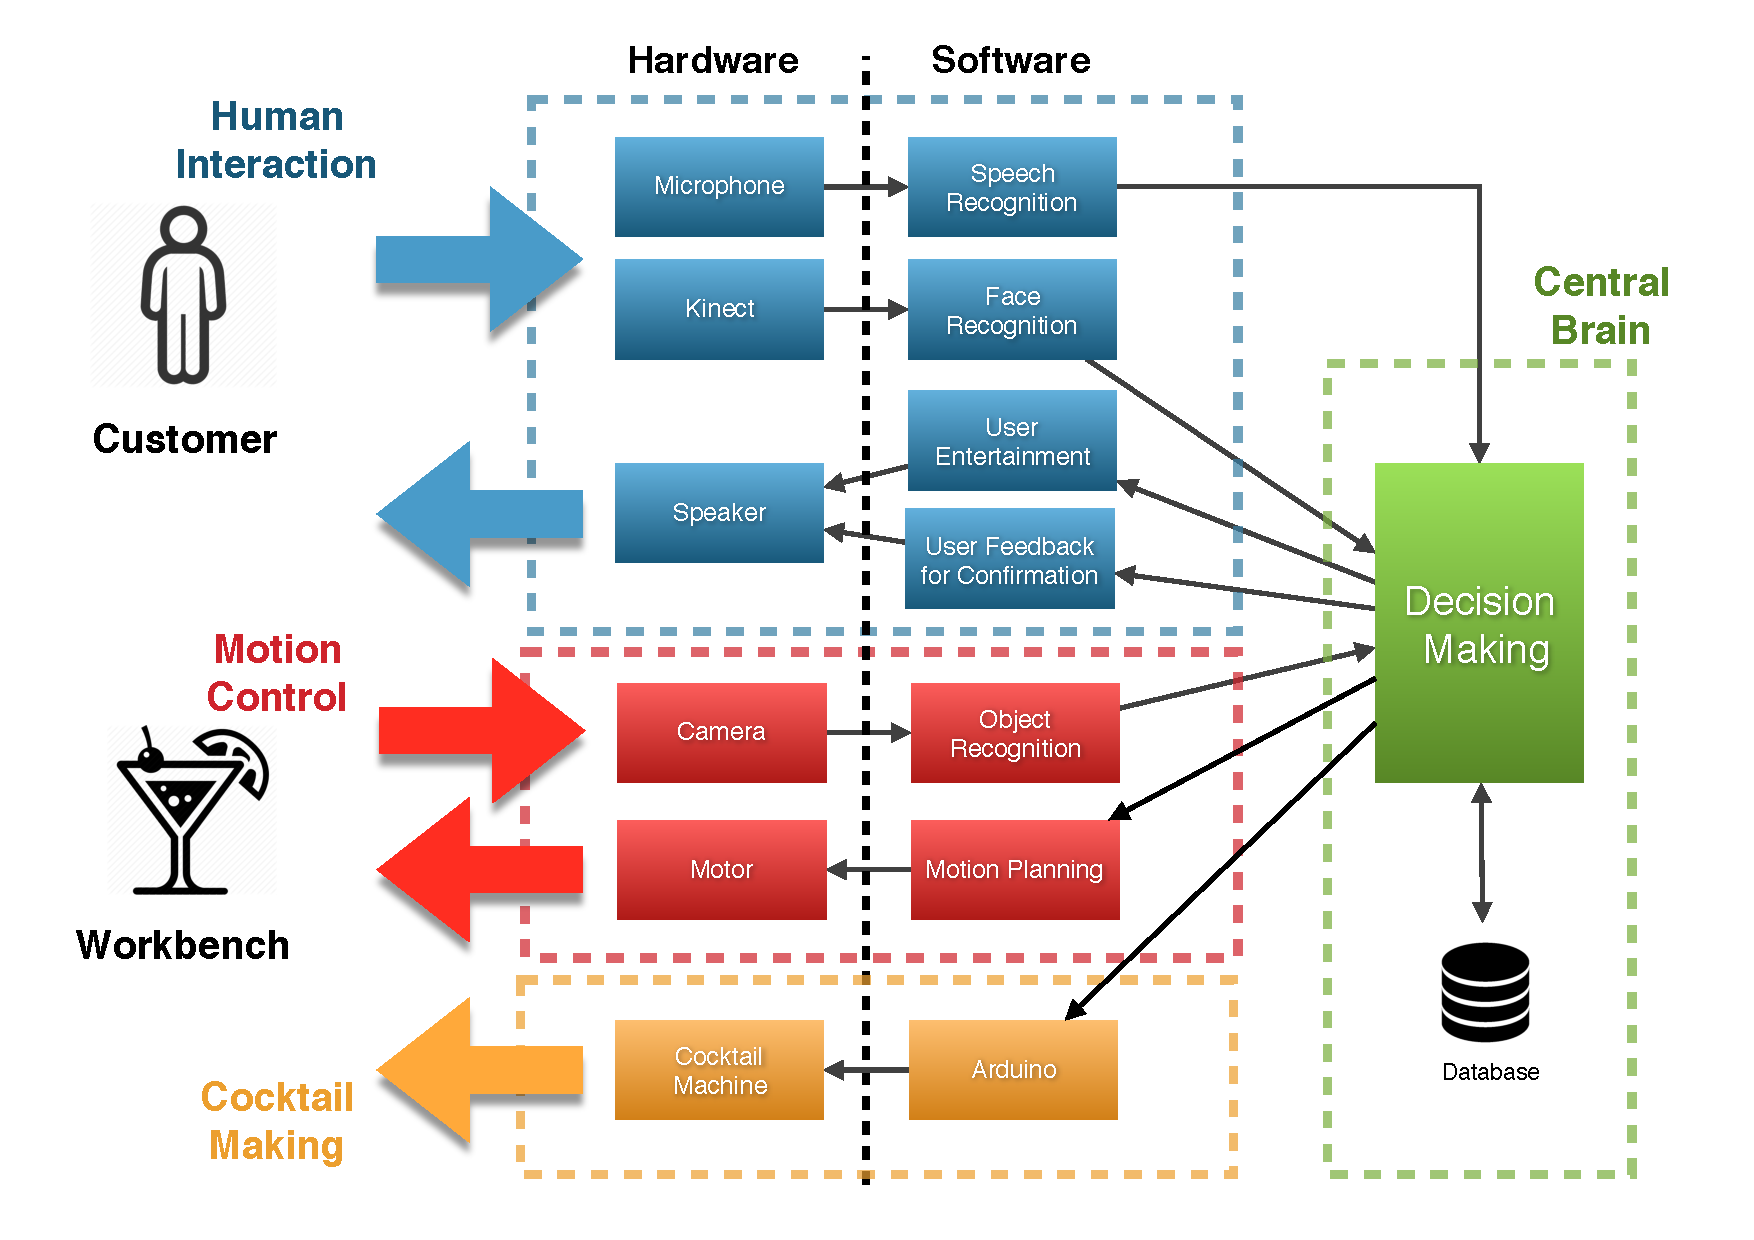
\includegraphics[width=0.45\textwidth]{figures/BlockDiagram}
	\caption{Smartini's functional blocks}
	\label{fig:blockDiagram}
\end{figure}


\subsection{Robot Functions}
\textit{Wysiwyd} -- `What You Say Is What You Did' is one of the most famous international projects that are currently dealing with Human-Robot Interaction. It aims to develop communication strategies between humans and robots based on biological behaviours, and to improve robotic skills in terms of learning from human verbal communication and body language. \textit{Wysiwyd} offers high-level APIs to perform complex tasks, and it provides modules to manage every aspect of the robot's interaction with the external environment. To achieve our goals (speech recognition, face/object detection/recognition, motion) we built on the work done by \textit{Wysiwyd} researchers. In what follows we discuss the main functions our our robot, and how we played with \textit{Wysiwyd} to obtain what we needed.

\subsubsection{Speech Recognition}
First speech recognition approaches for this project have been done with PocketSphinx.
It provides the the possibility to employ a grammar or a statistical language models in order to improve the speech recognition for a specific application \cite{SphinxLangModel}.

A grammar enables the creation of a structure for commands and word sequences in general. Possible words and phrases can be specified in order to increase the recognition accuracy significantly. Additionally, rules and optional words can be defined.
%However, strict grammars can trigger problems especially if the speech recognition system is used by people who are not familiar with the grammar. For example, if a required word of the grammar is skipped, the recognition fails completely.

A statistical language model defines words and phrases including a probability of occurrence. It can be generated automatically out of a list of possible sentences. If the speaker says a sentence that is not in this list but every word is, the sentence still can be recognised correctly. 
%In comparison to a grammar, a statistical language model permits the user to speak more freely and in an arbitrary pattern. This is well-suited for speakers who are unfamiliar with the speech recognition system.

Both methods were tested in environments with different background noises. 
Since the error rate increases as the number of different words in the grammar or the language model increases, a very small vocabulary was used. In a completely silent environment, the recognition accuracy was nearly 100\%. However, in a noisy environment, PocketSphinx was not able to differentiate between a voice and noise. Even with a reduced microphone sensitivity, the beginning and the ending of a spoken phrase was detected very badly and the recognition accuracy was very poor.

Finally, the Speech Application Programming Interface (SAPI) provided by Microsoft Windows was used for speech recognition in this project \cite{SAPI}. The problem of background noise was nearly completely overcome by the usage of a headset microphone with reduced sensitivity.

In order to achieve a high recognition performance, different grammars are employed depending on the words that are likely in the current context. For example, if the customer is asked whether he wants to have a cocktail, it is expected that his answer either includes the word `yes' or `no'. For the cocktail ordering process the grammar consists of the cocktail names and typical phases like `Can I have ... please' or `I want ... please'.

\subsubsection{Speech Synthesis}

Speech synthesis could also be carried over using the already implemented $say()$ function. However, \textit{wysywid} functions must complete before the next one can be called. This presented an issue for us, as we wanted to be able to move while talking. For this reason, we did not opt to use the pre-defined function, but rather found out how the text-to-speech worked at a lower level and exploited that. 

Speech synthesis happens over YARP via a module called $iSpeak$ \cite{gitspeech}. This module accepts a text-to-speech package as argument when it is run. After that, it will connect to the speaker of the machine onto which it is running, and turn incoming TCP string commands into sounds. 

Inside the brain module, we opened a port and connected it to $/iSpeak$ using YARP functions. This package may vary between machines. Popular ones are \emph{festival} and \emph{espeak} or the default ones for Windows and Mac OSX: \emph{speech-dev} and \emph{say}. 

A very simple custom $say()$ function was implemented to send bottled strings to such port. By doing so, we lost the pre-implemented feature (in \textit{Wysiwyd}) that moves the robot's mouth as it is speaking. However we felt that this was a good compromise as it allowed us to turn and move the robot's arms as he spoke. As future work, we could re-integrate the mouth feature. 

\subsubsection{Interaction} 

Communication had to be intuitive, since a cocktail-maker ultimately has to deal with constantly changing customers, who cannot be instructed in advance. Speech acts as a primary form of communication between humans and as such it is the most intuitive way for humans to communicate with our robot \cite{RobotsMeetHumans}. Therefore speech recognition and speech synthesis were used as the primary way to interact with the human user.

Interaction is performed in almost all of the states of the robot, as will be described more in detail in Section \ref{Architecture}. It is used to set up dialogues with the user, which are useful to greet the customer, understand the choice of cocktail, provide information and entertainment while preparing the drink, and gathering information from the user. 

\subsubsection{Object Recognition}

The visual system is one of the autonomous systems inside the \textit{Wysiwyd} environment, and it is of relevant interest in two areas: face detection and object detection and recognition.

The iCub is the ideal platform to undertake research in cognitive systems with various types of agents, and it's mounted on a six-degrees-of-freedom, controllable head. These cameras have a resolution of 320x240px and can stream at a 33Hz frame rate. 

Object localisation must be able to work reliably even while the robot is moving its eyes and or its upper body. Various local reference frames (e.g. 
the left and right eye frames) need to be continuously converted into the reference frame in which we want to express object locations. 

The key points for implementing object recognition are: 

\begin{itemize}
\item Location
\item Colour
\item Tag
\end{itemize}
	

The idea behind location-based recognition is to pre-define a range of positions where the objects can be placed on the workbench, to address the attention of the iCub in the right direction. This way, the robot does not need to check the whole area in front of itself, but only specific portions. 

To detect and segment objects from an image it is helpful to use objects having uniform colours. Moreover, objects and the background should have a significant colour difference.

It is also possible to identify an item using tags, so that an object (after being recognised) is given a name and, when requested, the iCub associates the tag to the selected object. To do this, we made use of OPC (\textit{objectsPropertiesCollector}), where all objects are created and insert in a database, with a specific name.

These `tricks' were not mandatory for the success of object recognition, but were adopted in our project to avoid developing complicated learning algorithms, which would have been beyond our scope. 

After implementing object recognition, we tested its reliability and found that a handful of extra precautions were needed. One of the main discriminating factors was the distance between the cameras and the objects. As lighting conditions varied throughout the day, further objects were picked up less reliably. Therefore, in the final design, we made sure critical objects were as close as possible to the iCub. Moreover, we observed that symmetrical objects were being recognised more reliably. This is due to the difference in appearance of non-symmetrical objects when seen from different angles. As such, we opted to use symmetrical, uniformly-coloured cups in our final implementation. 

\subsubsection{Human Detection and Recognition} \label{humanDetection}

Another crucial aspect of this project was human detection. Indeed, this feature was used as the first step to trigger all other process in our system, as discussed in Section \ref{Architecture}. We used a Kinect, located on the head of the iCub, to identify a customer and determine his distance and relative position. To enhance its compatibility, face detection was implemented with a pre-defined library, the \textit{iol2opc}, from the \textit{Wysiwyd} environment, so that the Kinect can communicate directly with the modules that run inside the iCub.

Some issues were exposed while testing this feature. As with the object recognition, one of the issues was the variation of light during the day, which could interfere with accurate detections. Moreover, we observed that due to the position and the height of the iCub, tall users could be out of the scope of Kinect. Furthermore, it had difficulty isolating one face among multiples in the same frame, therefore we limited our project to one customer at a time.

\subsubsection{Motion}
The overall motion system was already embedded into \textit{wysiwid} environment and it is based on ARE (\textit{Action Rendering Engine}), an iCub library which implements high-level motion instructions. Functions like \textit{points(target name)} or \textit{lookAt(target name)} are ready-to-use tools for our purposes, but their usage is strictly dependant on successful identification and labelling of objects and agents by the \textit{OPC} system. On other hand, protection against `objects/agents not found' are presents inside those functions, and, in the worst case scenario, the iCub will not perform the required action(for safety reasons). Since all of the objects needed for our project lie on the table in front of the iCub, it is important to keep a constant visual contact with them (in order to let OPC correctly updating their positions). The \textit{home()} function is used for this purpose, moving iCub robot to its starting position, from where the robot has the best possible perspective of the table. It is also good practice to call \textit{home()} to reset the position errors of all the joints accumulated during several sequential actions (mainly due to imprecise low-level PID motors control laws), and hence achieve more precision for the following movements. Moreover, particular attention is necessary when adopting the \textit{point()} function, especially when  `static' target points outside the workspace are initialized into the OPC table: if these object are too far, the iCub will stretch its torso and arm towards them, ending up in an unnatural position, endangering some of its joints. For this reason, it is always necessary to first `project' these far points onto a closer plane, by replacing the real position of the object with a closer `shadow' one. It is then possible to call the \textit{point()} function using one of those `shadow' points as argument.

\subsection{System Architecture} \label{Architecture}

\begin{figure}[h]
	\centering
	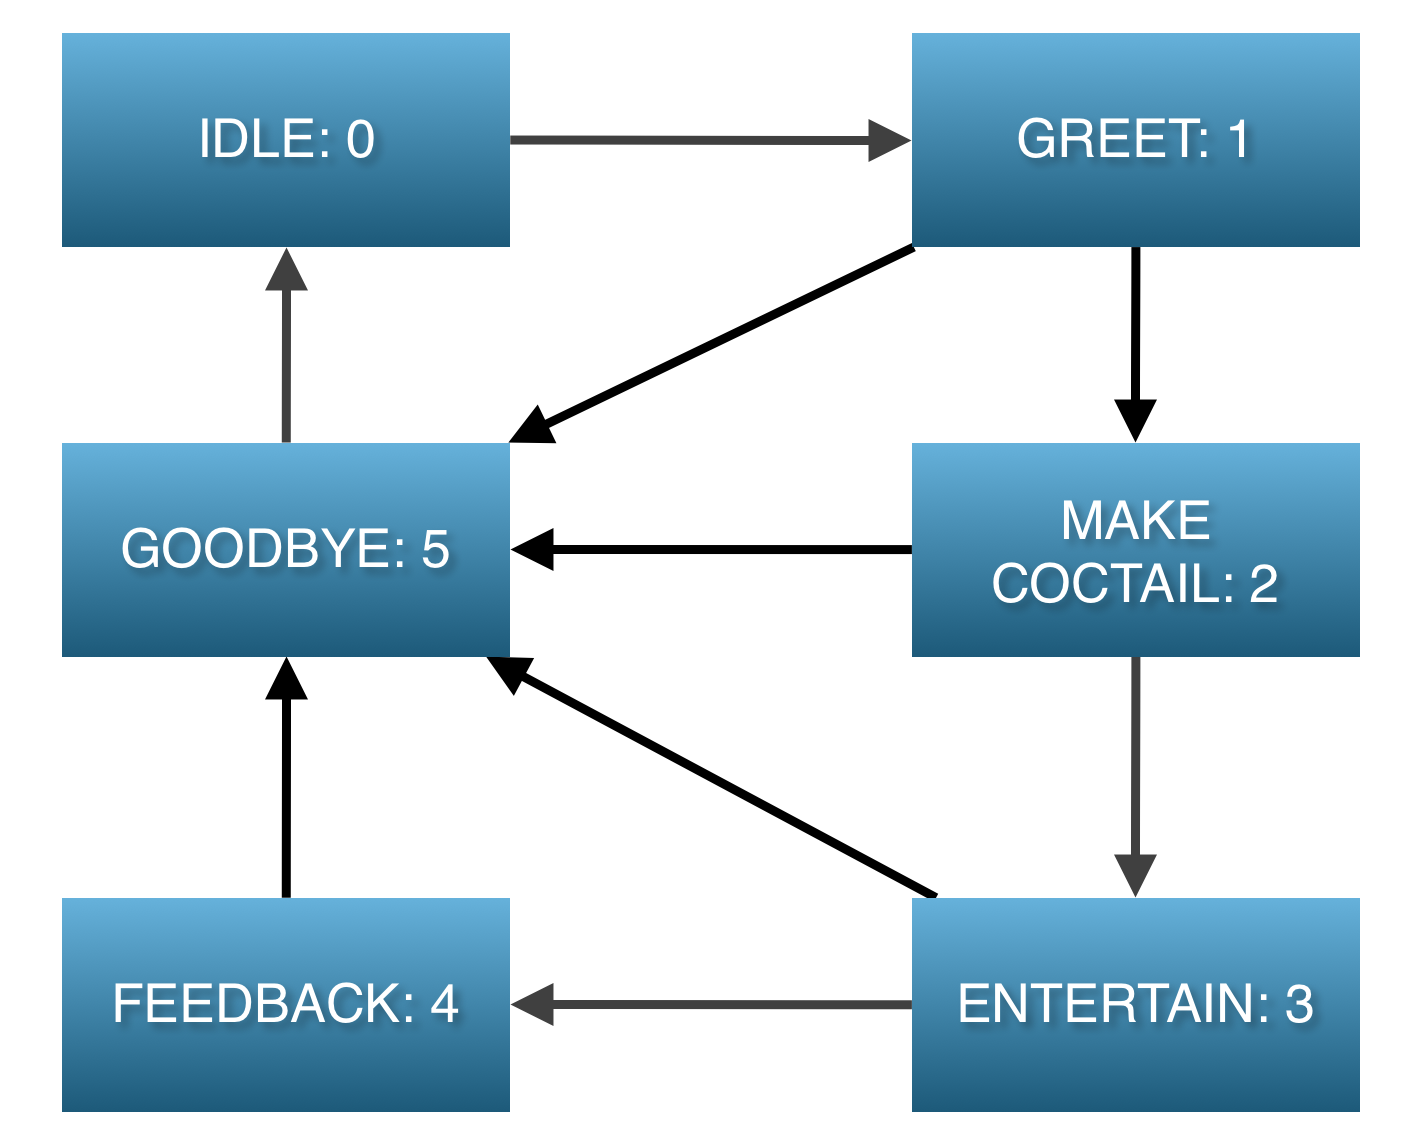
\includegraphics[width=0.3\textwidth]{figures/StateMachine}
	\caption{Core states of robot's architecture}
	\label{fig:stateMachine}
\end{figure}


The structure of the code was designed around a finite state machine. There are 6 main states, each with their own sub-states, which happen in sequence from when the robot recognises a potential customer to when it says goodbye. At any time, there are safety checks that reset the state machine to its idle state (after saying goodbye), to prevent getting stuck when something goes wrong. This overall structure is displayed in Figure \ref{fig:stateMachine} and is discussed in more detail in the following subsections. 

\subsubsection{Idle State}

The starting point of the system is the IDLE state, where the iCub waits for somebody to pass by. When someone arrives, the robot can detect the face of a new customer with a stereo vision system due to the Kinect on the head of the iCub.

As discussed in Section \ref{humanDetection}, the Kinect is integrated inside the overall system, so it could be easily interfaced with the rest of the program. This way, the code creates a new Agent object on the OPC database every time the robot sees a new customer, setting a variable called \textit{isPresent}, and moving on to the next state: GREET. From now on, the Agent field is updated in the background by the Kinect and accessible via OPC to the rest of the program. This is useful to fetch the user's position when needed (e.g. to look at him while talking) or to determine if he left and we need to return to the IDLE state. 

\subsubsection{Greet State}

If a customer is detected by the Kinect camera, Smartini will look at him and speak to introduce himself. After that, he asks the customer whether he wants to have a cocktail. If the customer answers yes, he is asked to choose a cocktail from the menu. In order to avoid a misunderstanding, Smartini repeats the recognised cocktail name and asks for confirmation.
Should anything go wrong (e.g. the customer left), or if the customer prefers not to get a cocktail, Smartini says good bye and returns to the idle state.

\subsubsection{Make Cocktail State}

For this step, object recognition plays a major role. On entering this state, the OPC database is filled with all the objects that are present on the workbench, so that the iCub can later identify them. 

We adopted two object types in our project: static and dynamic. With static objects, we only need the object's location. For example, Smartini might want to indicate a topping to add to the drink by pointing at it. With dynamic objects, such as glasses, we expect their position to change during the cocktail-making process. 

When the object initialisation is completed, Smartini asks the customer to take a glass and put it under the Smartini Machine. While the robot is talking to the customer, it simultaneously indicates the glass that the customer needs to pick up (stored under \textit{'starting\_position'} on OPC) and where to put it (stored under \textit{'final\_position'} on OPC). The iCub is capable (with a certain tolerance) to check if the glass was placed in the appropriate position, and based on that it will ask the customer to move it, or it will continue with the cocktail preparation. As a safety measure, Smartini only asks three more times to move the glass to the right position before the state is changed to GOODBYE.

 \begin{figure}[h]
	\centering
	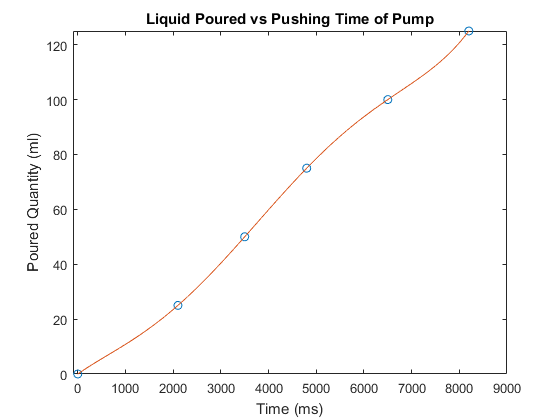
\includegraphics[width=0.35\textwidth]{figures/interpolation_pumps.png}
	\caption{Flow chart for cocktail feedback}
	\label{fig:interpolation}
\end{figure} 

When the glass is recognised at the correct position, the cocktail recipe is scanned and ingredient quantities (in ml) are retrieved. Then, an instruction containing a pair (ingredient/quantity) is created and sent to Arduino via Serial Port. Between an instruction and next one, the iCub leaves the Home position, looks at the costumer and explains how much of each ingredient is being poured into the glass. At the same time, Arduino unpacks the received signal and it maps the ingredient index and the quantity of liquid to, respectively, the pump number and the pushing time (in millisecond) for the pump. Figure \ref{fig:interpolation} shows the function used to get the correct mapping between quantity(in ml) and pushing time, and it has been produced interpolating several measurements(represented by circles in the figure). When the pouring phase is finished, the iCub asks the customer to add some topping on the cocktail (retrieved from the recipe as well), and then it moves to the ENTERTAIN state. 

\subsubsection{Entertain State}

The entertainment is carried out with two simple approaches. The first one consists in generating expressions and jokes from the robot, relating to the role of a bartender as well as playing around with its robot nature. This part is meant to be funny and engaging for the user, easing the interaction with a machine by making it more human-like. Bartenders are commonly recognised as someone you can talk to, and customers often bring up their personal problems to them \cite{bartenderPsy}. Here we would like to simulate this human side, by hinting in a humorous way at this aspect of being a bartender.
The second approach keeps the user entertained by reading news from the internet. This was implemented by reading off the titles of an article to the customer after using expressions such as ``Did you know that today'' or ``Have you heard that'' and then concluding with others like ``How cool is that?'' or ``At first I thought it was a joke''. The delivered version of the software pre-stores the news in the same way as the jokes (described above), however this was not the original plan. Our strategy was to fetch this information on the spot, via RSS (Rich Site Summary), which is provided freely by most news agencies and can be used to fetch the titles of the most popular articles as well as categorize them into topics \cite{bbcRss}. Fetching RSS feeds is done widely, and it uses XML parsers. Multiple libraries were tested, but we eventually delivered a static version due to cross-compatibility issues and time constraints. As future work, this would be something worth integrating in the project. 


\subsubsection{Feedback State}

 \begin{figure}
	\centering
	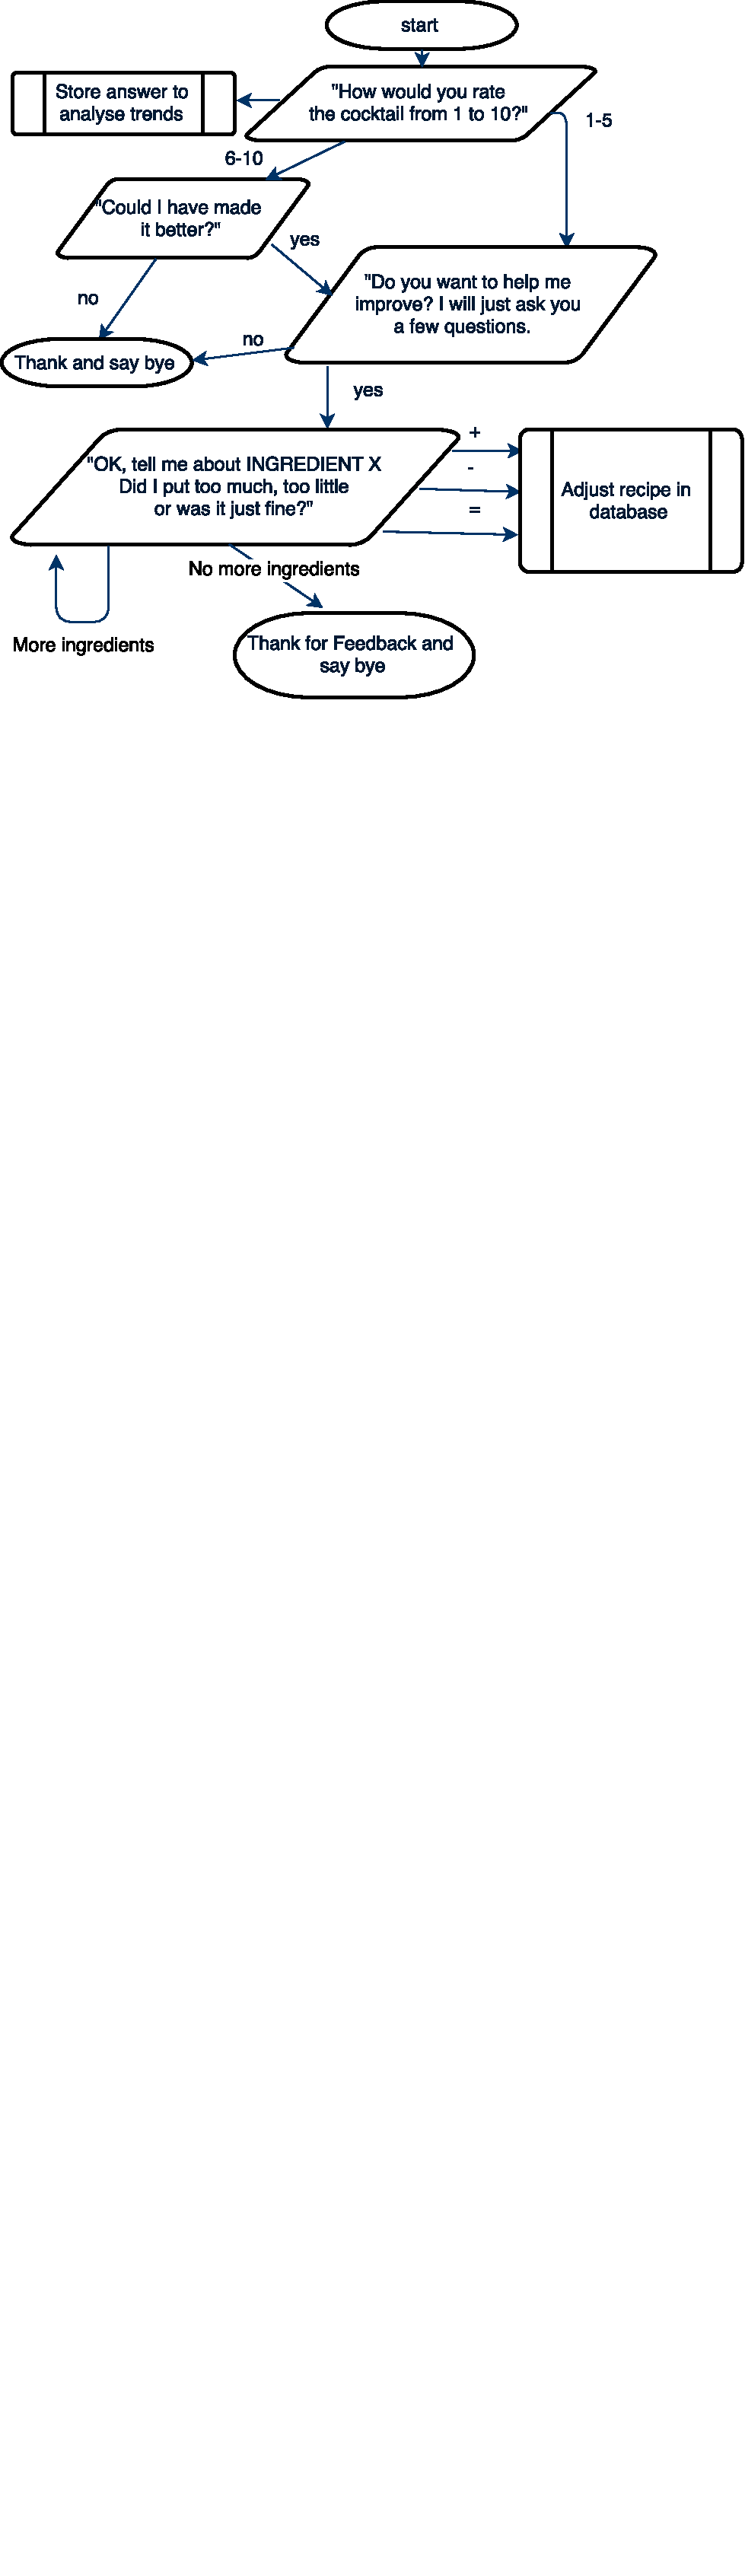
\includegraphics[width=0.4\textwidth]{figures/feedback}
	\caption{Flow chart for cocktail feedback}
	\label{fig:feedback}
\end{figure} 

After the cocktail is ready, Smartini asks questions to the user to assess the quality of the beverage and learn how to make a better cocktail from what the user says. For simplicity, these questions imply short answers, such as yes or no or numerical values. The feedback state can be considered a finite state machine on its own, and its structure is represented in Figure \ref{fig:feedback}. As shown, the programme is structured to fetch two types of information: a vote on the cocktail and a comment on the quantity of its ingredients. Smartini remembers the comments from previous customers when making the same cocktail again. With this feature, we expect the votes to show a positive trend, meaning that Smartini successfully learnt how to adjust its recipes to human taste. 

Every time a user thinks that there was too much or too little of a particular ingredient, the new adjusted recipe is saved onto a file. This file is then loaded when booting Smartini, so that previous knowledge is never lost and the trends can be observed across multiple test runs. 

\subsubsection{Goodbye State}
In the last state of this state machine, Smartini says good bye and wishes the customer a nice day. Afterwards, Smartini returns to the IDLE state.

\subsection{Cocktail Machine}

\subsubsection{Hardware}

	\begin{itemize}
    
     	\begin{figure}
		\centering
		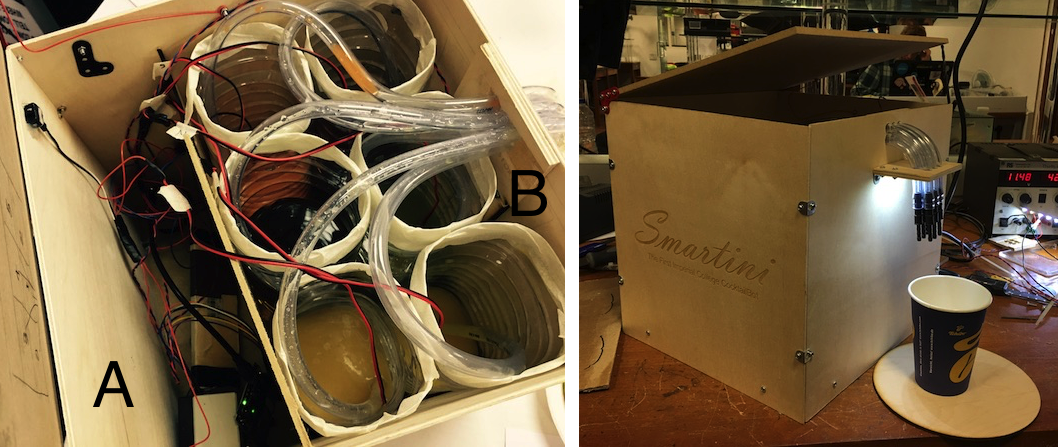
\includegraphics[width=0.4\textwidth]{figures/boxCollaged}
		\caption{Top and Side views of Smartini Machine}
		\label{fig:box}
		\end{figure}
    
		\item Box\\From the outside, the Smartini Box is a 30x30x30cm cube made out of wood. Internally, it consists of two compartments. As shown in Fig. \ref{fig:box}, compartment A holds all the electronic components including an Arduino and a breadboard with a circuit which controls the pumps.
        
        In compartment B, it encloses 6 big bottles as ingredient reservoirs. Each one has a water pump immersed in it. The tubes are also all equal in length to prevent any inconsistency in portion size. These pumps are directly controlled by an Arduino which is in turn receive high-level commands from the iCub. 
            
    	\begin{figure}
		\centering
		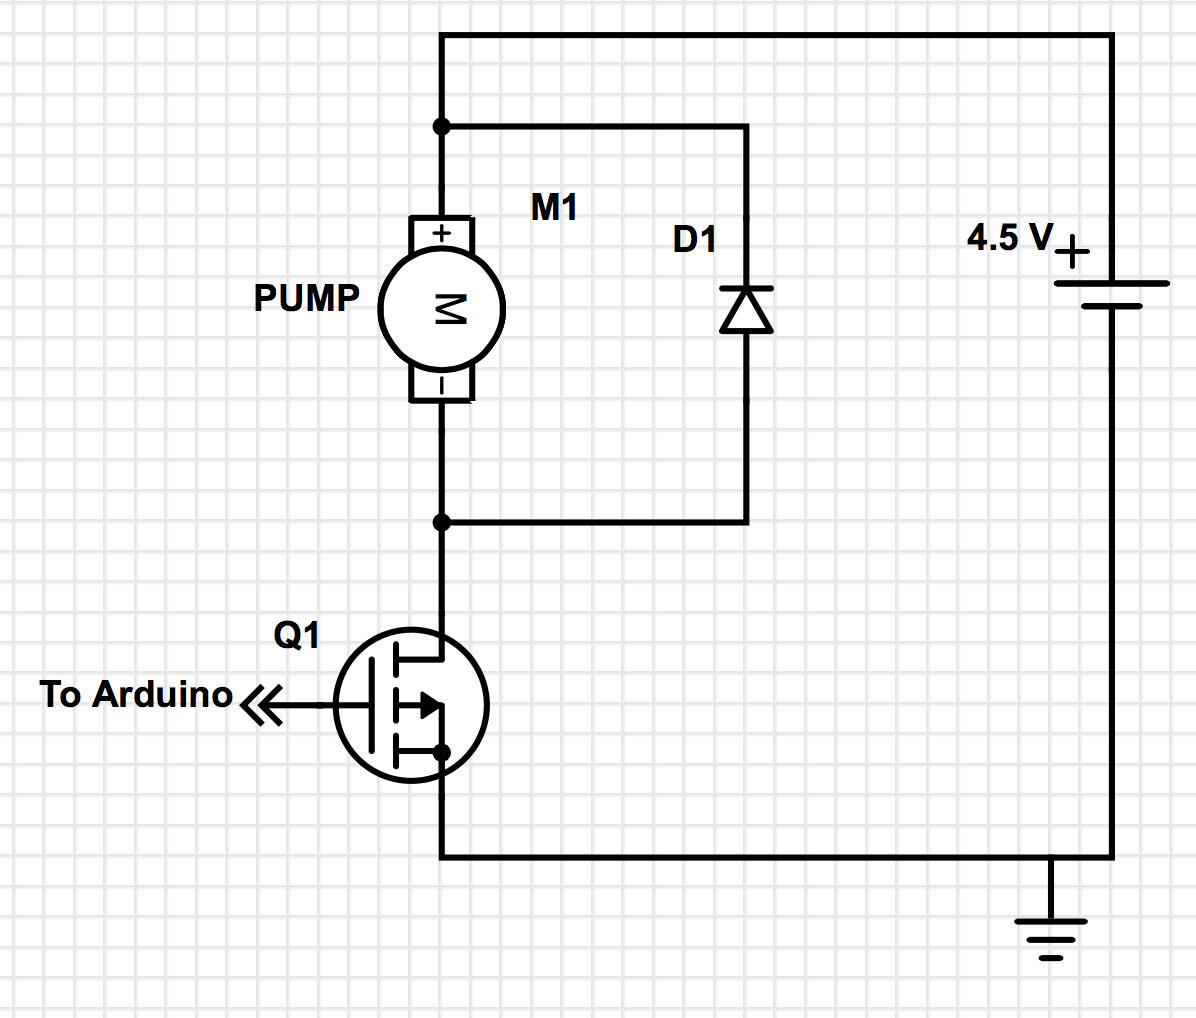
\includegraphics[width=0.3\textwidth]{figures/pumpCircuit}
		\caption{Pump driver circuit schematic}
		\label{fig:pumpCircuit}
		\end{figure} 
            
        \item Pumps \& Circuits\\The pumps can be treated as simple DC motors, and the basic circuit used to drive them is displayed in Fig. \ref{fig:pumpCircuit}. Thanks to their high flow rate, immersion pumps were used instead of peristaltic pump (our first choice). The value of the supply voltage was chosen to result in an ideal flow rate of the liquids (in terms of ml per second) for our purposes.
        
	\end{itemize}

\subsubsection{Software}
An Arduino Module is created on Yarp network with the purpose to link the Brain Module to the Arduino board. A Serial Port is opened by Arduino Module, and a check on the connection between Arduino board and Arduino module is done. Arduino board code is very simple: it polls until a string pair (ingredient index, quantity in ml) is received. Then it casts those values to integer type, it maps them into the correct pair(pump number, opening time in ms) according to the function in Fig. \ref{fig:interpolation}. Finally Arduino opens the gate of chosen MOSFET to activate the pump and add ingredients into the glass.
\section{Testing}

\subsection{Experimental Procedure}

The testing phase was more problematic than we had anticipated. We were not allowed to move the iCub from its position in the research lab, which means we had to convince users to come to the lab instead of bringing it to crowded places. Considering the timing of the testing phase, when most students have exams or pressing deadlines, convincing people to follow us was not an easy task. 

Moreover, the iCub was also being used for other research projects, an expert supervisor had to be with us while we used it. All of this mean that the actual available time of the iCub was very limited, and while the development phase was carried out primarily using simulators, testing needed the robot. 

Due to all this, we were only able to run tests with 18 users. Clearly, the sample was not large enough to have strong statistical meaning, but we could still draw some conclusions about Smartini's performance. In what follows, we will discuss what we consider partial results, and further tests should be performed should this project be passed on to future students. 

The test consisted in a full cycle with a customer. Smartini would identify when a customer approached his workbench, and initiate an interaction followed by the preparation of a cocktail, user entertainment and feedback gathering. Each cycle would take about 7 to 10 minutes to complete. 

At the end of the test, the customers were asked to fill in a survey to evaluate the performance of the various components of the Smartini. This questionnaire aimed to assess Smartini's performance in both making the cocktail and interacting with the customers. 

\subsection{Results}

The average votes for the Interaction section were the following:

\begin{itemize}
\item 
Telling Jokes:  \hfill 3.77
\item 
Reading News:  \hfill 3.00
\item 
Cocktail-Making Process:  \hfill 4.23
\item 
Feedback Gathering:  \hfill 4.08
\item 
Robot's Movements:  \hfill 3.54
\item 
Robot's Eye-Contact:  \hfill 3.54
\item 
Easiness of Communication:  \hfill 3.54

\end{itemize}

In terms of the cocktail performance, Fig. \ref{fig:ingResults} displays the curves obtained with the two most popular cocktails. Here we can observe how the ingredient quantities were altered according to user feedback, and how the rating of the same cocktails changed accordingly. 

\begin{figure}[t!]
    \centering
    \begin{subfigure}[t]{0.25\textwidth}
        \centering
        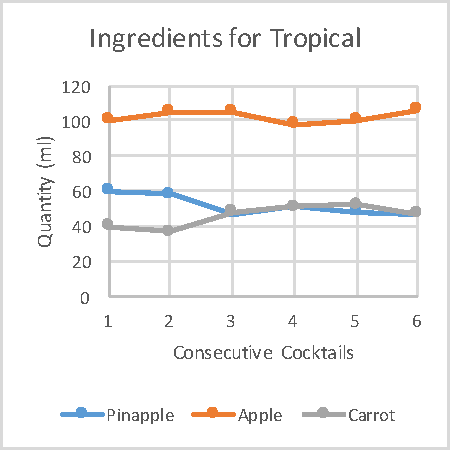
\includegraphics[height=1.6in]{figures/tropicalIng}
%         \caption{}
    \end{subfigure}%
    ~ 
    \begin{subfigure}[t]{0.25\textwidth}
        \centering
        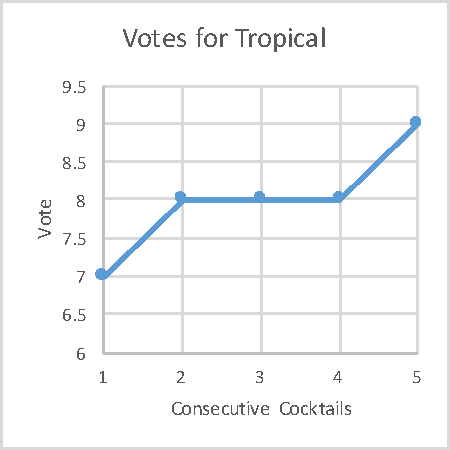
\includegraphics[height=1.6in]{figures/tropicalVotes}
    \end{subfigure}
        \begin{subfigure}[t]{0.25\textwidth}
        \centering
        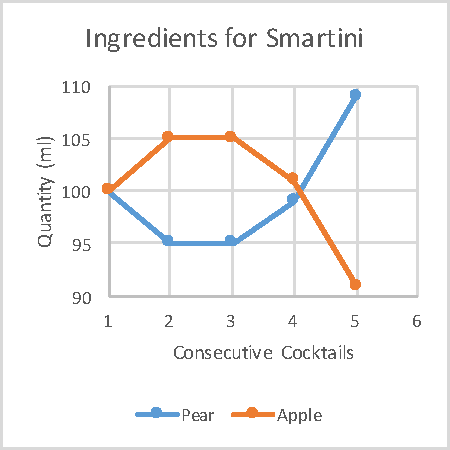
\includegraphics[height=1.6in]{figures/smartiniIng}
    \end{subfigure}%
    ~ 
    \begin{subfigure}[t]{0.25\textwidth}
        \centering
        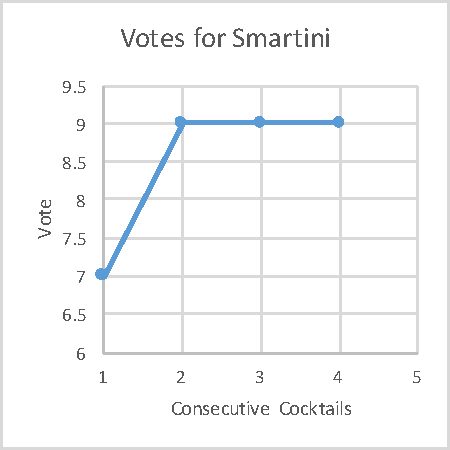
\includegraphics[height=1.6in]{figures/smartiniVotes}
    \end{subfigure}
    \caption{Cocktail ingredients evolution and relative votes}
    \label{fig:ingResults}
\end{figure}

\section{Observations}

Overall Smartini obtained high marks for its interaction skills, never dropping below 3 out of 5 for any sub-component. This was very satisfactory since the interaction was the focus of our exercise. Moreover, colloquial jokes and expressions had a better impact than impersonal news reading. This seems to confirm our second hypothesis. We can attest that, when dealing with imperfect machines, humans seem to appreciate a type of interaction that acknowledges the robotic nature of the machine, and jokes around it instead of hiding it. 

Smartini received slightly lower marks for its movements and eye-contact. Unfortunately, safety reasons forced us to limit its movements to a minimum, which probably affected this part of the tests. Interestingly, the easiness of communication seems strongly correlated with eye-contact and movements, which would confirm our third hypothesis. Should this trend be reconfirmed with a higher testing sample, we could conclude that gesticulations and eye-contact are central for a successful and enjoyable human-robot interaction, as we proposed in our third hypothesis. 

As with the evolution of the cocktails, the numbers are unfortunately too low to draw strong conclusion, despite 4 out of 5 available cocktails showing positive trends. From this part, however, we can appreciate the successful mechanism to gather the feedback (which received the overall highest mark) and alter the cocktail recipe. Should this project be passed on, it will surely start with a strong ground. 

\section{Future Work}

\subsection{Human detection}

Originally, our idea was to include face recognition in our work. However, no existing libraries are currently implemented to approach this task, and with our limited time we did not feel that it was appropriate to work on our own. For the future, it would be useful to port an OpenCV library on the YARP environment, with its face detection tools. Moreover, It would be of interest obtain the possibility to engage more than one customer at the same time, like a real bartender could do.

\subsection{Object detection and recognition}

To build the computational equivalent of a human mind, it is necessary to obtain a robust perception of the environment. Our colour-based object-recognition methods work under strict assumptions about the lighting and background (preferably a white table or a wall), and they generally fail in cluttered settings. To help our robot, we shaped our testing environment so that when the Smartini was required identify an object, the most distinguishing feature was simply the fact that the object of interest was closer to the robot than the background. Nevertheless, it was not easy to find methods for depth estimation from a stereo pair which were a good trade-off between robustness (e.g. to lighting conditions) and speed, two requirements that are key for working in real world robotic scenarios. Should this project be passed on to another group, we would strongly recommend investing in a more robust object recognition system, which was not our priority, but would be crucial for a fully functional bartender robot. 



\section{Conclusion}

Overall, the design of Smartini was a success. We were forced to a couple of strategy changes along the way, but we can claim to have successfully found alternatives and we were able to deliver a system that effectively understands orders, prepares cocktails with accurate ingredient quantities, entertains its customers, gathers feedback from them and learns to improve its recipes. We relied on pre-existing tools, but we also explored new techniques, which allowed for example to perform concurrent tasks such as talking and moving at the same time (not currently possible using \textit{wysisyd}). The testing phase was below our expectations due to reasons partly beyond our control, yet we could still draw some useful conclusions and partially confirm some of our hypotheses. 


% Can use something like this to put references on a page
% by themselves when using endfloat and the captionsoff option.
\ifCLASSOPTIONcaptionsoff
  \newpage
\fi



% trigger a \newpage just before the given reference
% number - used to balance the columns on the last page
% adjust value as needed - may need to be readjusted if
% the document is modified later
%\IEEEtriggeratref{8}
% The "triggered" command can be changed if desired:
%\IEEEtriggercmd{\enlargethispage{-5in}}

% references section

% can use a bibliography generated by BibTeX as a .bbl file
% BibTeX documentation can be easily obtained at:
% http://www.ctan.org/tex-archive/biblio/bibtex/contrib/doc/
% The IEEEtran BibTeX style support page is at:
% http://www.michaelshell.org/tex/ieeetran/bibtex/
%\bibliographystyle{IEEEtran}
% argument is your BibTeX string definitions and bibliography database(s)
%\bibliography{IEEEabrv,../bib/paper}
%
% <OR> manually copy in the resultant .bbl file
% set second argument of \begin to the number of references
% (used to reserve space for the reference number labels box)
\begin{thebibliography}{1}
	
	
\bibitem{stats}
``Service Robotics - Global Industry Analysts, Inc.'' Service Robotics (MCP-6565) - Global Industry Analysts, Inc. (2016)
\emph{http://www.strategyr.com/Service\_Robotics\_Market\_Report.asp}

\bibitem{stats2}
``Service Robot Statistics.'' IFR RSS. (2016)
\emph{http://www.ifr.org/service-robots/statistics/}


\bibitem{socialBots}
Fong, Terrence, Illah Nourbakhsh, and Kerstin Dautenhahn. ``A survey of socially interactive robots.'' Robotics and autonomous systems 42.3 (2003): 143-166.

\bibitem{engagement}
Sidner, Candace L., et al. ``Explorations in engagement for humans and robots.'' Artificial Intelligence 166.1 (2005): 140-164.


\bibitem{mmodal}
Kollar, Thomas, et al. ``A multi-modal approach for natural human-robot interaction.'' International Conference on Social Robotics. Springer Berlin Heidelberg, 2012.

\bibitem{valeria}
Gockley, Rachel, et al. ``Designing robots for long-term social interaction." 2005 IEEE/RSJ International Conference on Intelligent Robots and Systems. IEEE (2005).


\bibitem{petRobot}
Fujita, Masahiro. ``On activating human communications with pet-type robot AIBO." Proceedings of the IEEE 92.11 (2004): 1804-1813.

\bibitem{pouringLiquids}
\emph{https://www.youtube.com/watch?v=gthnQg153h4}

\bibitem{RobotsMeetHumans}
B. Jensen, ``Robots Meet Humans - Interaction in Public Spaces."
IEEE (2005).

\bibitem{gitspeech}
Robotology. ``Robotology/speech." GitHub. N.p., 2016. Web. 17 Nov. 2016. \emph{https://github.com/robotology/speech}

\bibitem{bartenderPsy}
Cowen, Emory L., Barbara J. McKim, and Roger P. Weissberg. ``Bartenders as informal, interpersonal." American Journal of Community Psychology 9.6 (1981): 715-729.

\bibitem{bbcRss}
News, BBC. ``News feeds from the BBC." BBC News. N.p., 2011. Web. 19 Dec. 2016. \emph{http://www.bbc.com/news/10628494}

\bibitem{c1} J. Gibson, Perceiving, Acting, and Knowing: Toward an Ecological
Psychology. Lawrence Erlbaum. (1977): 67–82.

\bibitem{c2}  M. Rudinac, G. Koostra, D. Kragic, and P. Jonker, ``Learning and
recognition of objects inspired by early cognition,” IEEE/RSJ Int. Conf. on Intelligents Robots and Systems. (2012)


\bibitem{c3} H. van Hoof, O. Kroemer, H. Ben Amor, and J. Peters, ``Maximally informative interaction learning for scene exploration," IEEE/RSJ Conf. on Intelligent Robots and Systems. (2012)


\bibitem{c4} P. Fitzpatrick, G. Metta, L. Natale, S. Rao, and G. Sandini, ``Learning
about objects through action - initial steps towards artificial cognition," in IEEE Int. Conf. on Robotics and Automation. (2003): 3140–3145.

\bibitem{c5} P. Fitzpatrick, A. Needham, L. Natale, and G. Metta, ``Shared challenges
in object perception for robots and infants," Infant and Child Development. (2008): 7–24

\bibitem{c6} R. Rouanet, P.-Y. Oudeyer, and D. Filliat, ``An integrated system for
teaching new visually grounded words to a robot for non-expert users using a mobile device," in IEEE-RAS Int. Conf. on Humanoid Robots, Tsukuba, Japan. (2009)

\bibitem{c7} M. Fiala, ``Artag, a fiducial marker system using digital techniques," in
IEEE Computer Society Conference on Computer Vision and Pattern
Recognition (CVPR), vol. 2, (2005): 590–596


\bibitem{c8} P. Viola and M. J. Jones, ``Robust real-time face detection," Int. J.
Comput. Vision, vol. 57. (2004): 137–154

\bibitem{c9}J. Fritsch, S. Lang, M. Kleinehagenbrock, G. A. Fink, and G. Sagerer,
“Improving adaptive skin color segmentation by incorporating results from face detection,” in IEEE Int. Workshop on Robot and Human Interactive Communication. (2002): 337–343

\bibitem{Sphinx1988}
Lee, K-F., and H-W. Hon. ``Large-vocabulary speaker-independent continuous speech recognition using HMM." Acoustics, Speech, and Signal Processing, 1988. ICASSP-88., 1988 International Conference on. IEEE (1988)

\bibitem{Sphinx1990}
Kai-Fu Lee, Hsiao-Wuen Hon, and Raj Reddy. ``An Overview of the {SPHINX} Speech Recognition System." IEEE Transactions on Acoustics, Speech, and Signal Processing 38.1 (1990): 35-45.

\bibitem{PocketSphinx}
Huggins-Daines, David, et al. ``Pocketsphinx: A free, real-time continuous speech recognition system for hand-held devices." 2006 IEEE International Conference on Acoustics Speech and Signal Processing Proceedings. Vol. 1. IEEE (2006)

\bibitem{SRhistory}
Biing-Hwang Juang and Lawrence R. Rabiner. ``Automatic Speech Recognition -- A Brief History of the Technology Development." Georgia Institute of Technology. Atlanta Rutgers University and the University of California. Santa Barbara 1 (2005): 67

\bibitem{speechLP}
Atal, Bishnu S., and Suzanne L. Hanauer. ``Speech analysis and synthesis by linear prediction of the speech wave." The Journal of the Acoustical Society of America 50.2B (1971): 637-655.

\bibitem{SRTechn}
Doda, Er Shweta, and Er Rajni Mehta. ``Speech Recognition Techniques: A Review." JCD Vidyapeeth, Sirsa, India 4.8 (2014).

\bibitem{SphinxLangModel}
``CMUSphinx." Building Language Model [CMUSphinx Wiki]. Carnegie Mellon University, n.d. Web. 18 Dec. 2016. \emph{http://cmusphinx.sourceforge.net/wiki/tutoriallm}


\bibitem{SAPI}
``Speech API Overview (SAPI 5.4)." N.p., n.d. Web. 20 Dec. 2016. \emph{https://msdn.microsoft.com/en-us/library/ee125077(v=vs.85).aspx}


\end{thebibliography}

% biography section
% 
% If you have an EPS/PDF photo (graphicx package needed) extra braces are
% needed around the contents of the optional argument to biography to prevent
% the LaTeX parser from getting confused when it sees the complicated
% \includegraphics command within an optional argument. (You could create
% your own custom macro containing the \includegraphics command to make things
% simpler here.)
%\begin{biography}[{\includegraphics[width=1in,height=1.25in,clip,keepaspectratio]{mshell}}]{Michael Shell}
% or if you just want to reserve a space for a photo:

\begin{IEEEbiography}[{\includegraphics[width=1in,height=1.25in,clip,keepaspectratio]{picture}}]{John Doe}
\blindtext
\end{IEEEbiography}

% You can push biographies down or up by placing
% a \vfill before or after them. The appropriate
% use of \vfill depends on what kind of text is
% on the last page and whether or not the columns
% are being equalized.

%\vfill

% Can be used to pull up biographies so that the bottom of the last one
% is flush with the other column.
%\enlargethispage{-5in}



% that's all folks
\end{document}



